\section{Конденсируй-умножай}
Рассмотрим уравнение конденсатора:
\begin{equation}
    I = C\frac{dU}{dt} = C\dot{U}
\end{equation}
Запишем его в виде передаточной функции:
\begin{equation}
    W(s) = \frac{1}{Cs}
\end{equation}
Получаем идеальное интегрирующее звено.
\subsection{Временные характеристики}
\noindent Найдем весовую функцию системы:
\begin{equation}
    y_{\text{i.r.}}(t) = L^{-1}\left\{\frac{1}{Cs}\right\} = \frac{1}{C} 
\end{equation}
Найдем переходную функцию:
\begin{equation}
    y_{\text{s.r.}}(t) = L^{-1}\left\{\frac{1}{Cs}\cdot\frac{1}{s}\right\} = \frac{t}{C} 
\end{equation}
Построим графики весовой (см. рис. \ref{fig:task3_impulse_response_eq}) и переходной (см. рис. \ref{fig:task3_step_response_eq}) функций.
\begin{figure}[ht!]
    \centering
    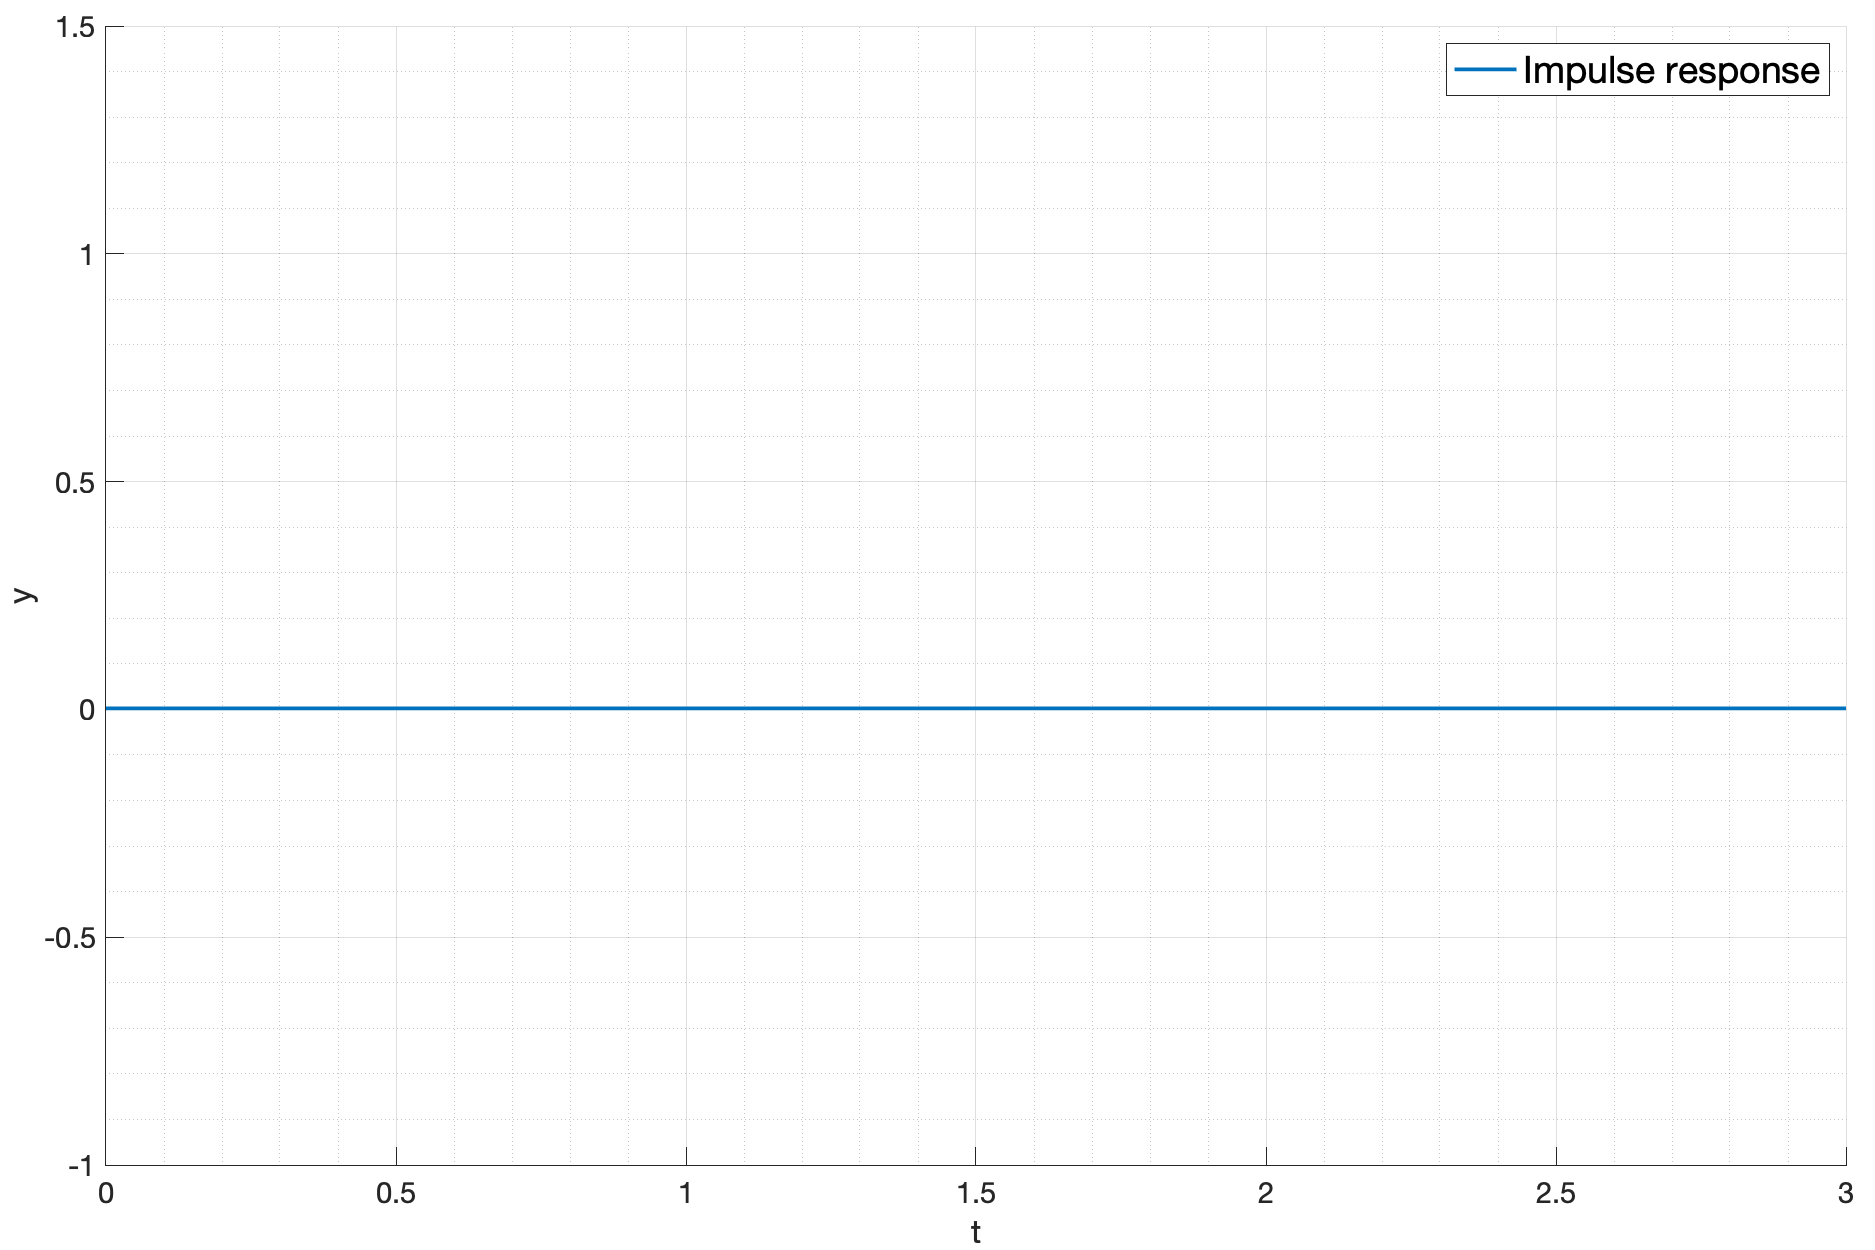
\includegraphics[width=\textwidth]{media/plots/task3_impulse_response_eq.png}
    \caption{Весовая функция конденсатора (теоретически)}
    \label{fig:task3_impulse_response_eq}
\end{figure}
\begin{figure}[ht!]
    \centering
    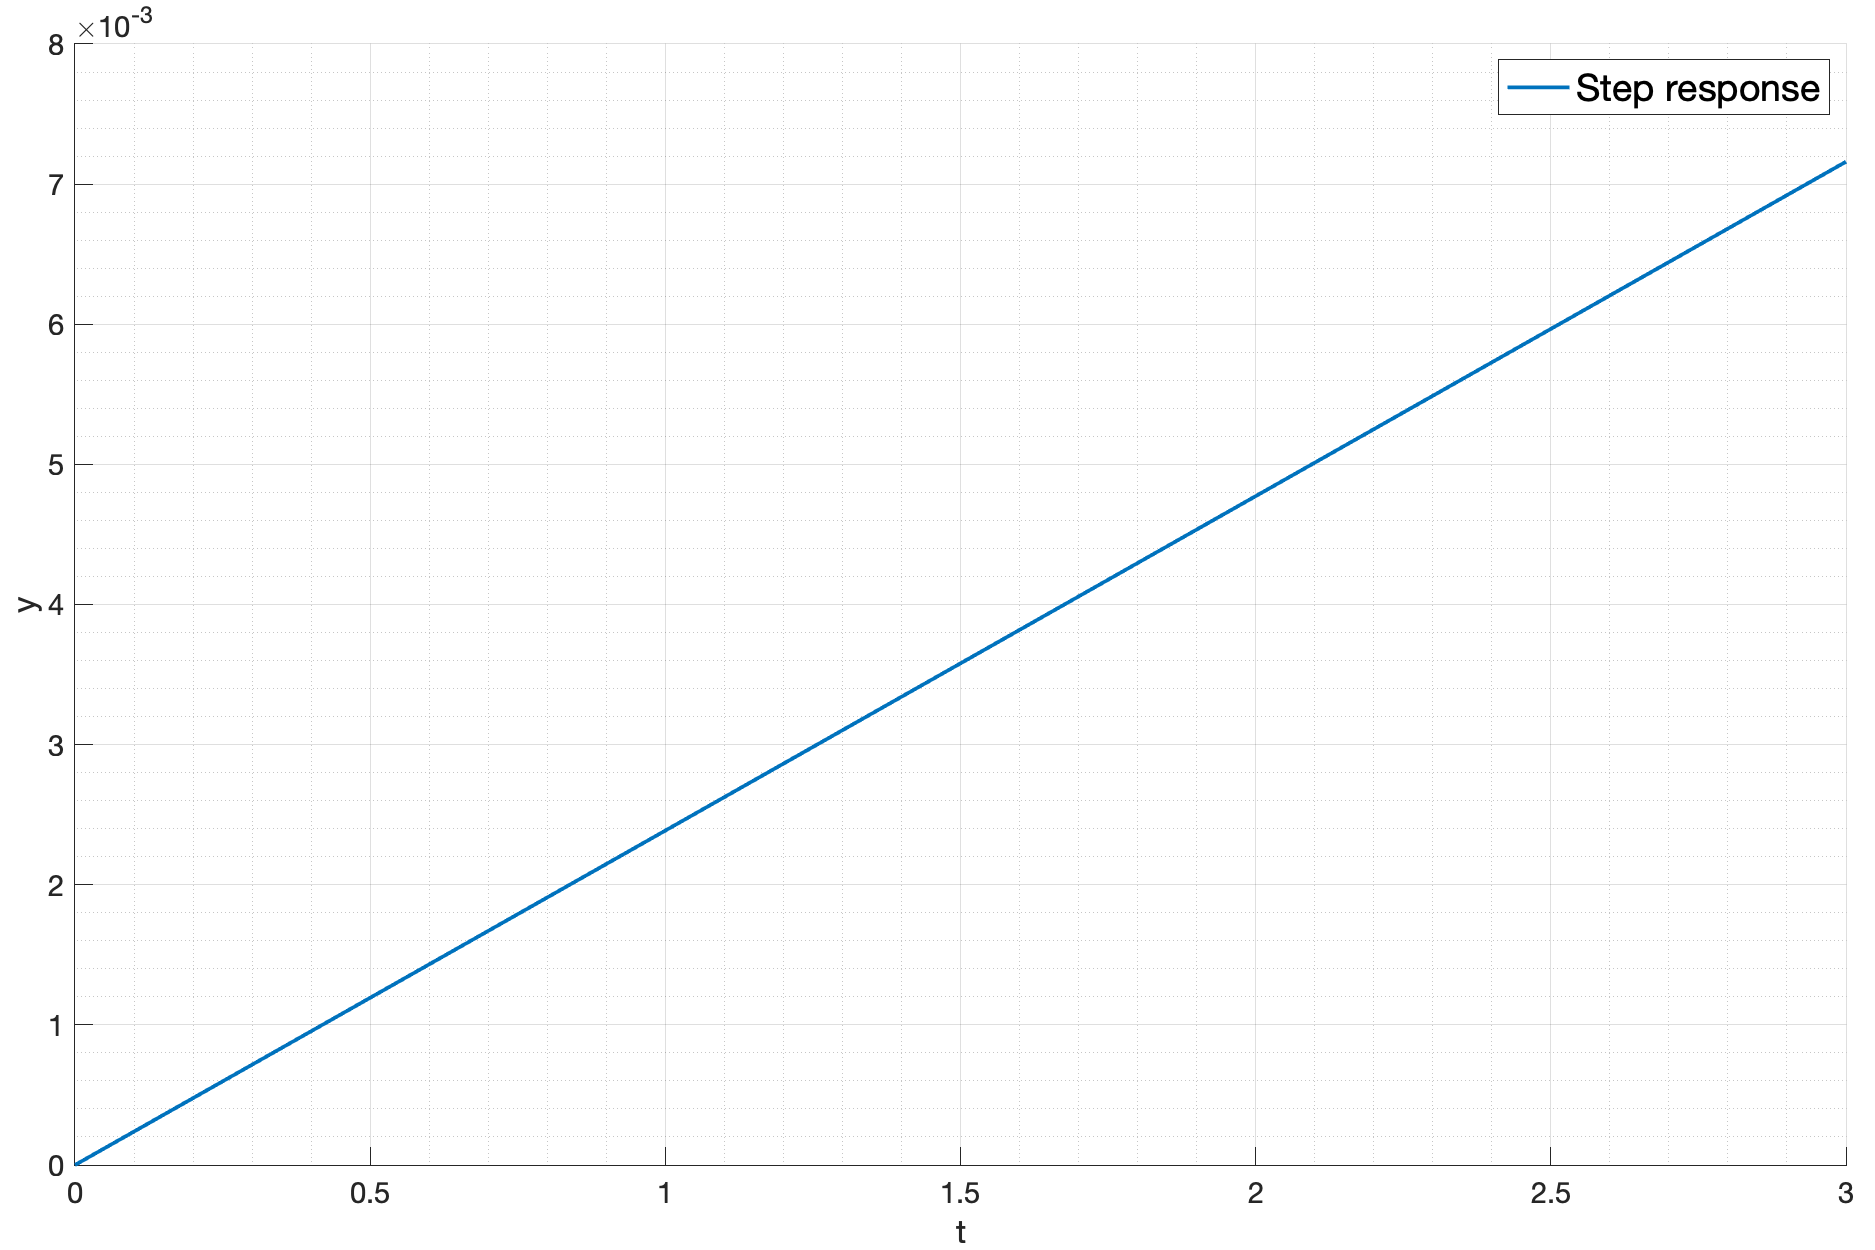
\includegraphics[width=\textwidth]{media/plots/task3_step_response_eq.png}
    \caption{Переходная функция конденсатора (теоретически)}
    \label{fig:task3_step_response_eq}
\end{figure}

Весовая (см. рис. \ref{fig:task3_impulse_response_exp}) и переходная (см. рис. \ref{fig:task3_step_response_exp}) функции, полученные в результате моделирования:
\begin{figure}[ht!]
    \centering
    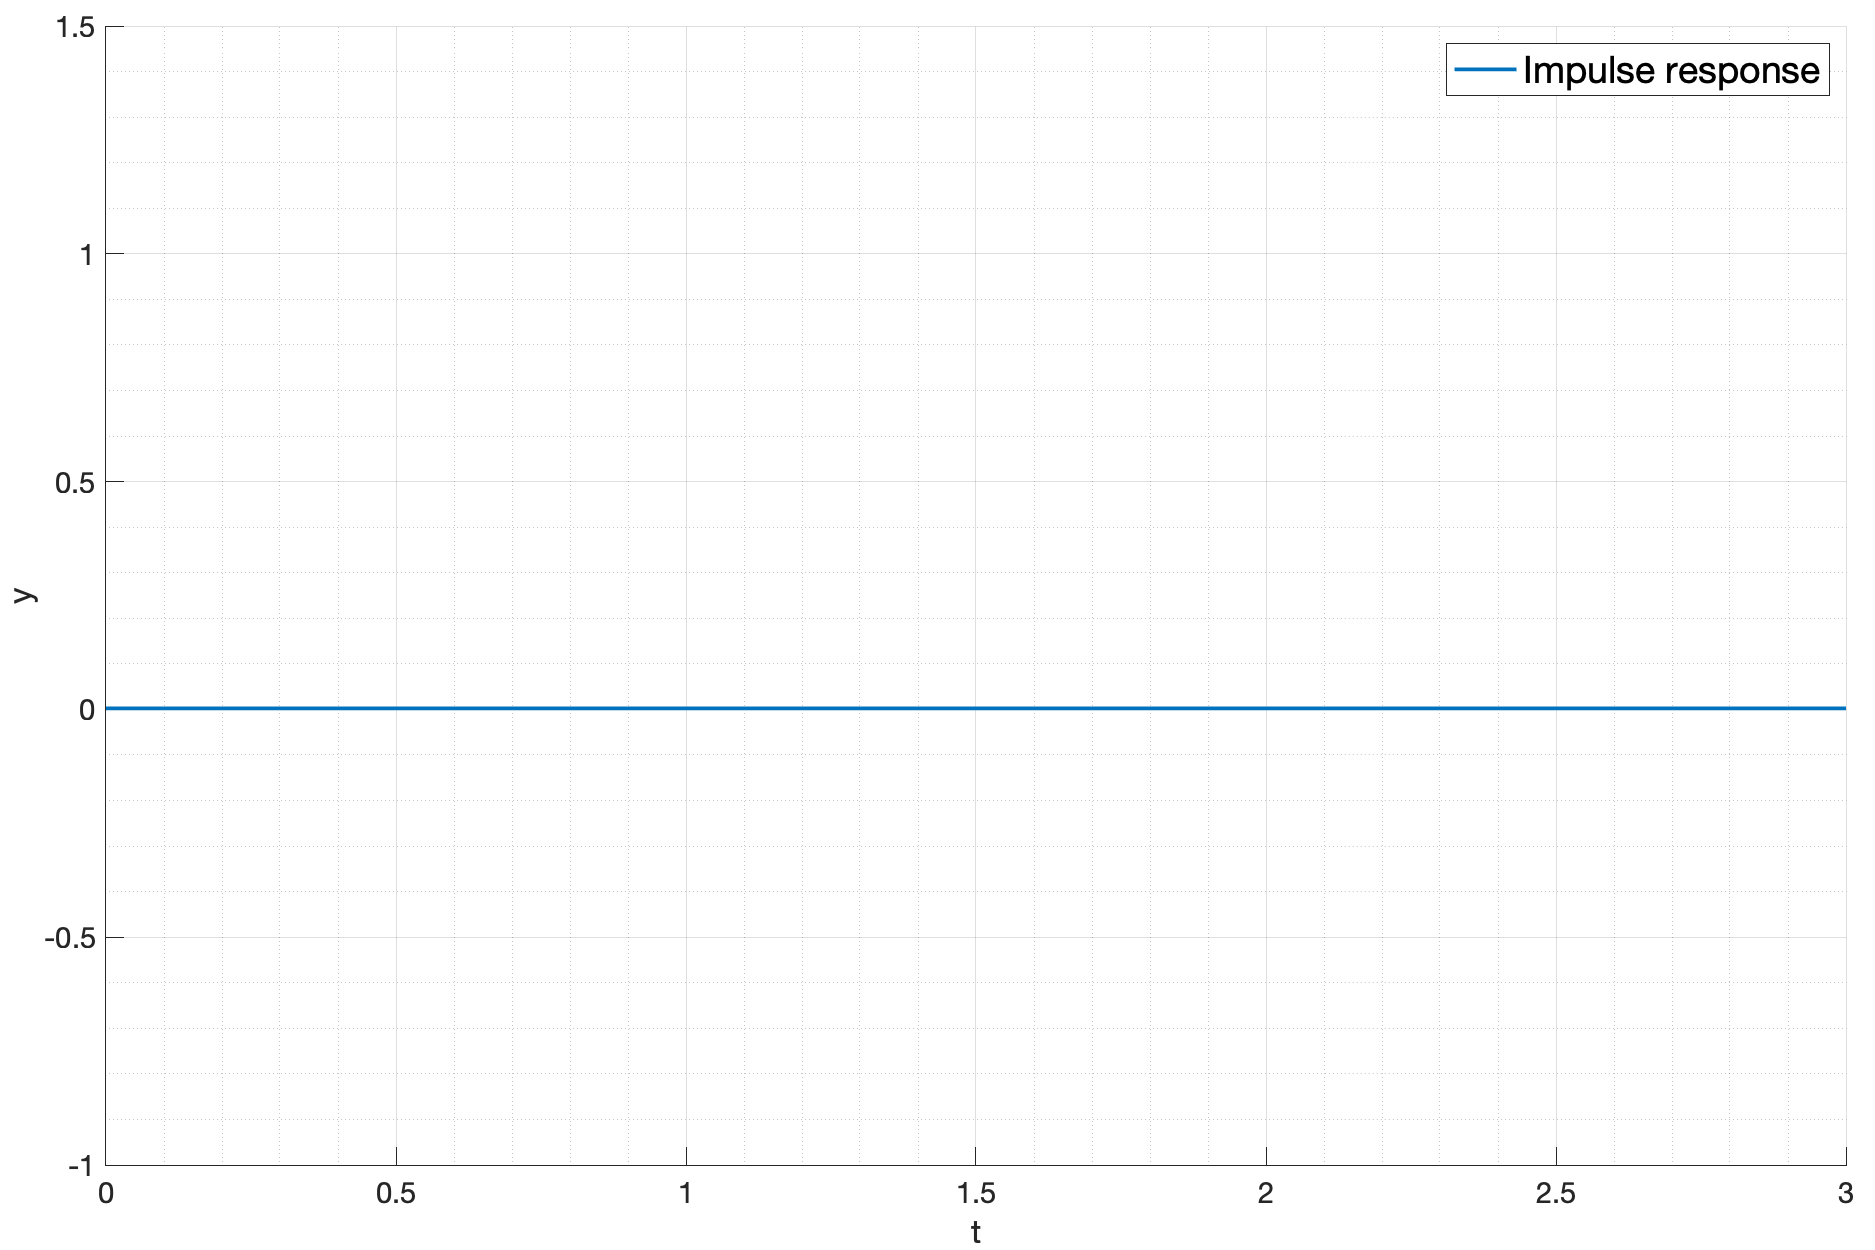
\includegraphics[width=\textwidth]{media/plots/task3_impulse_response_exp.png}
    \caption{Весовая функция конденсатора (экспериментально)}
    \label{fig:task3_impulse_response_exp}
\end{figure}
\begin{figure}[ht!]
    \centering
    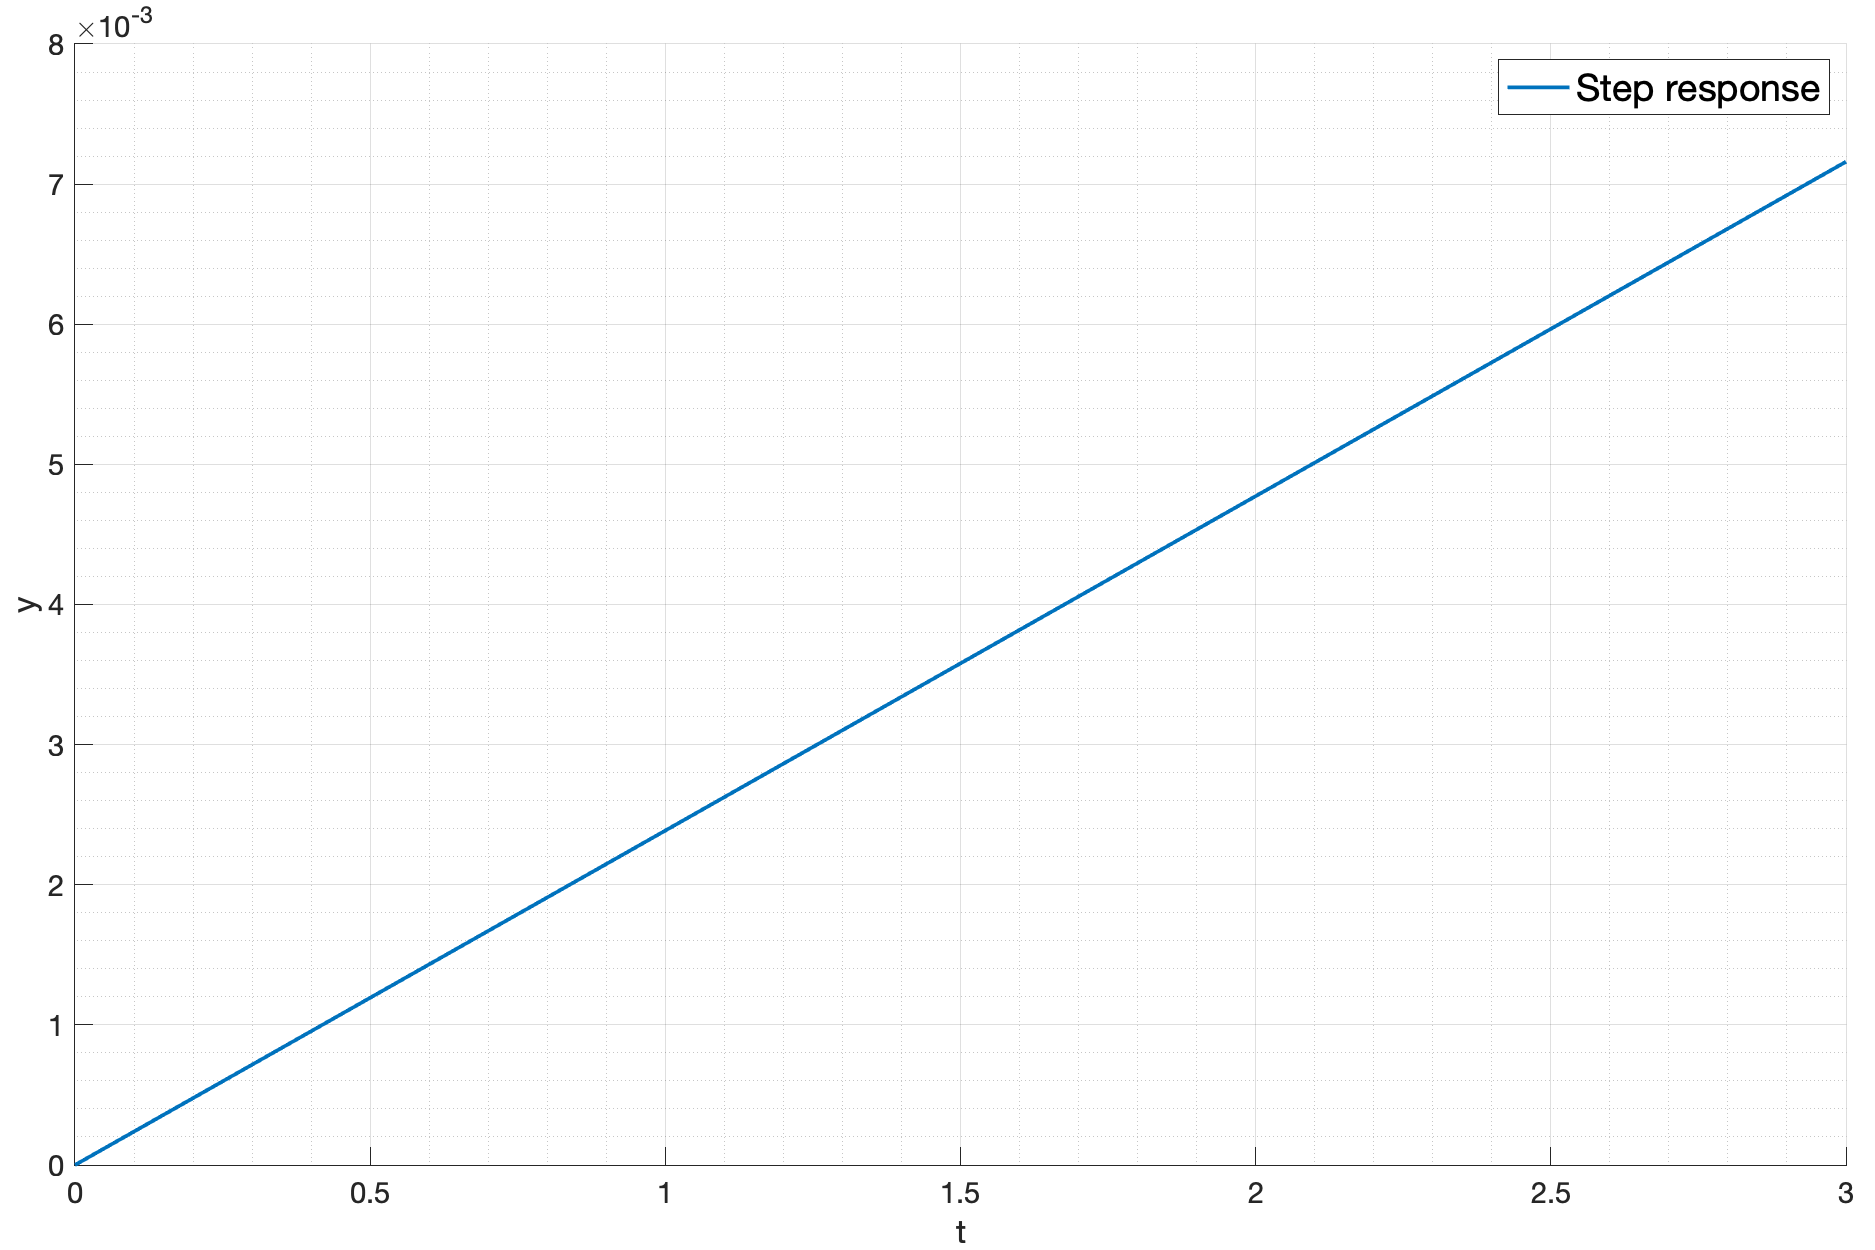
\includegraphics[width=\textwidth]{media/plots/task3_step_response_exp.png}
    \caption{Переходная функция конденсатора (экспериментально)}
    \label{fig:task3_step_response_exp}
\end{figure}

Сравнительные графики приведены на рис. \ref{fig:task3_impulse_response_cmp} и рис. \ref{fig:task3_step_response_cmp}.
\begin{figure}[ht!]
    \centering
    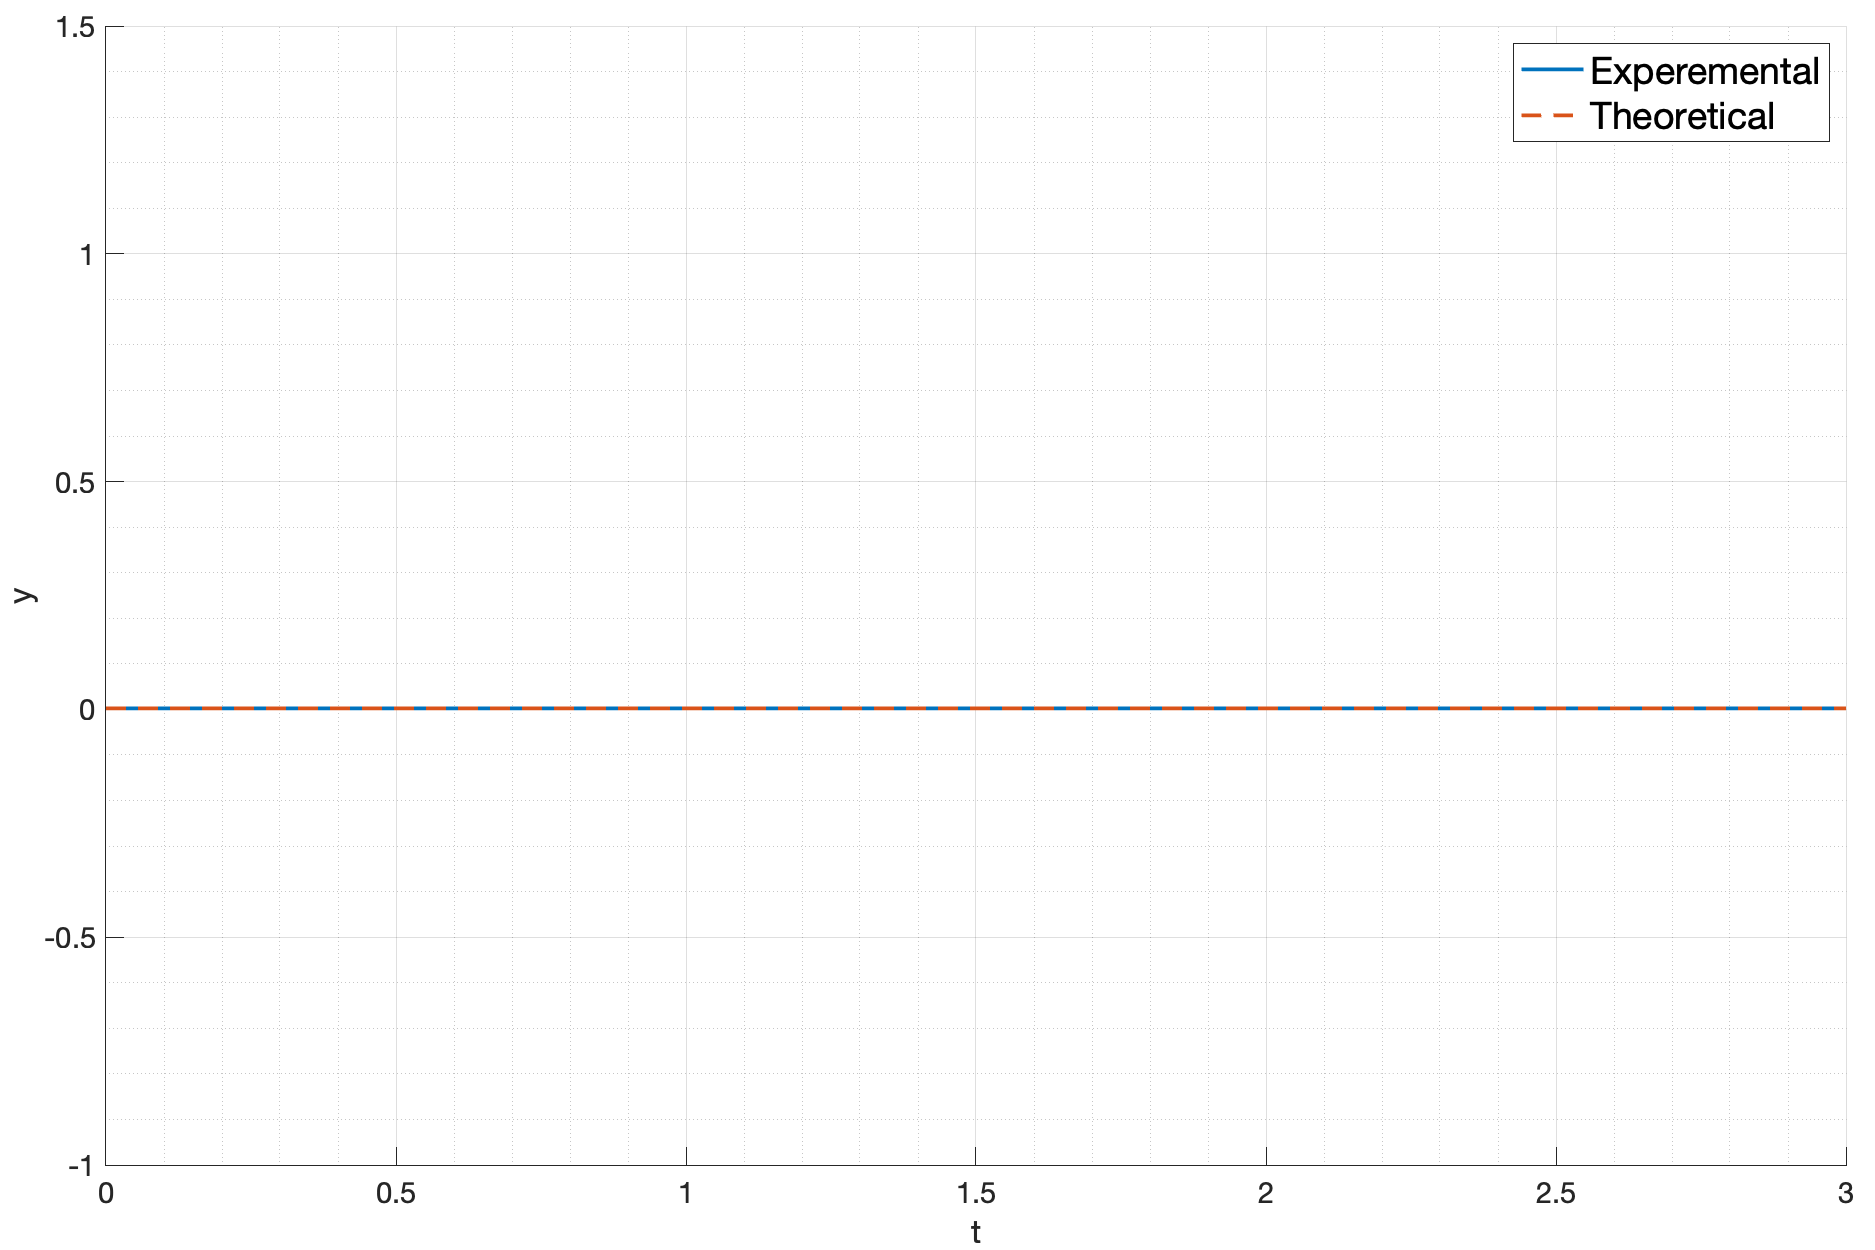
\includegraphics[width=\textwidth]{media/plots/task3_impulse_response_cmp.png}
    \caption{Сравнение весовых функций конденсатора}
    \label{fig:task3_impulse_response_cmp}
\end{figure}
\begin{figure}[ht!]
    \centering
    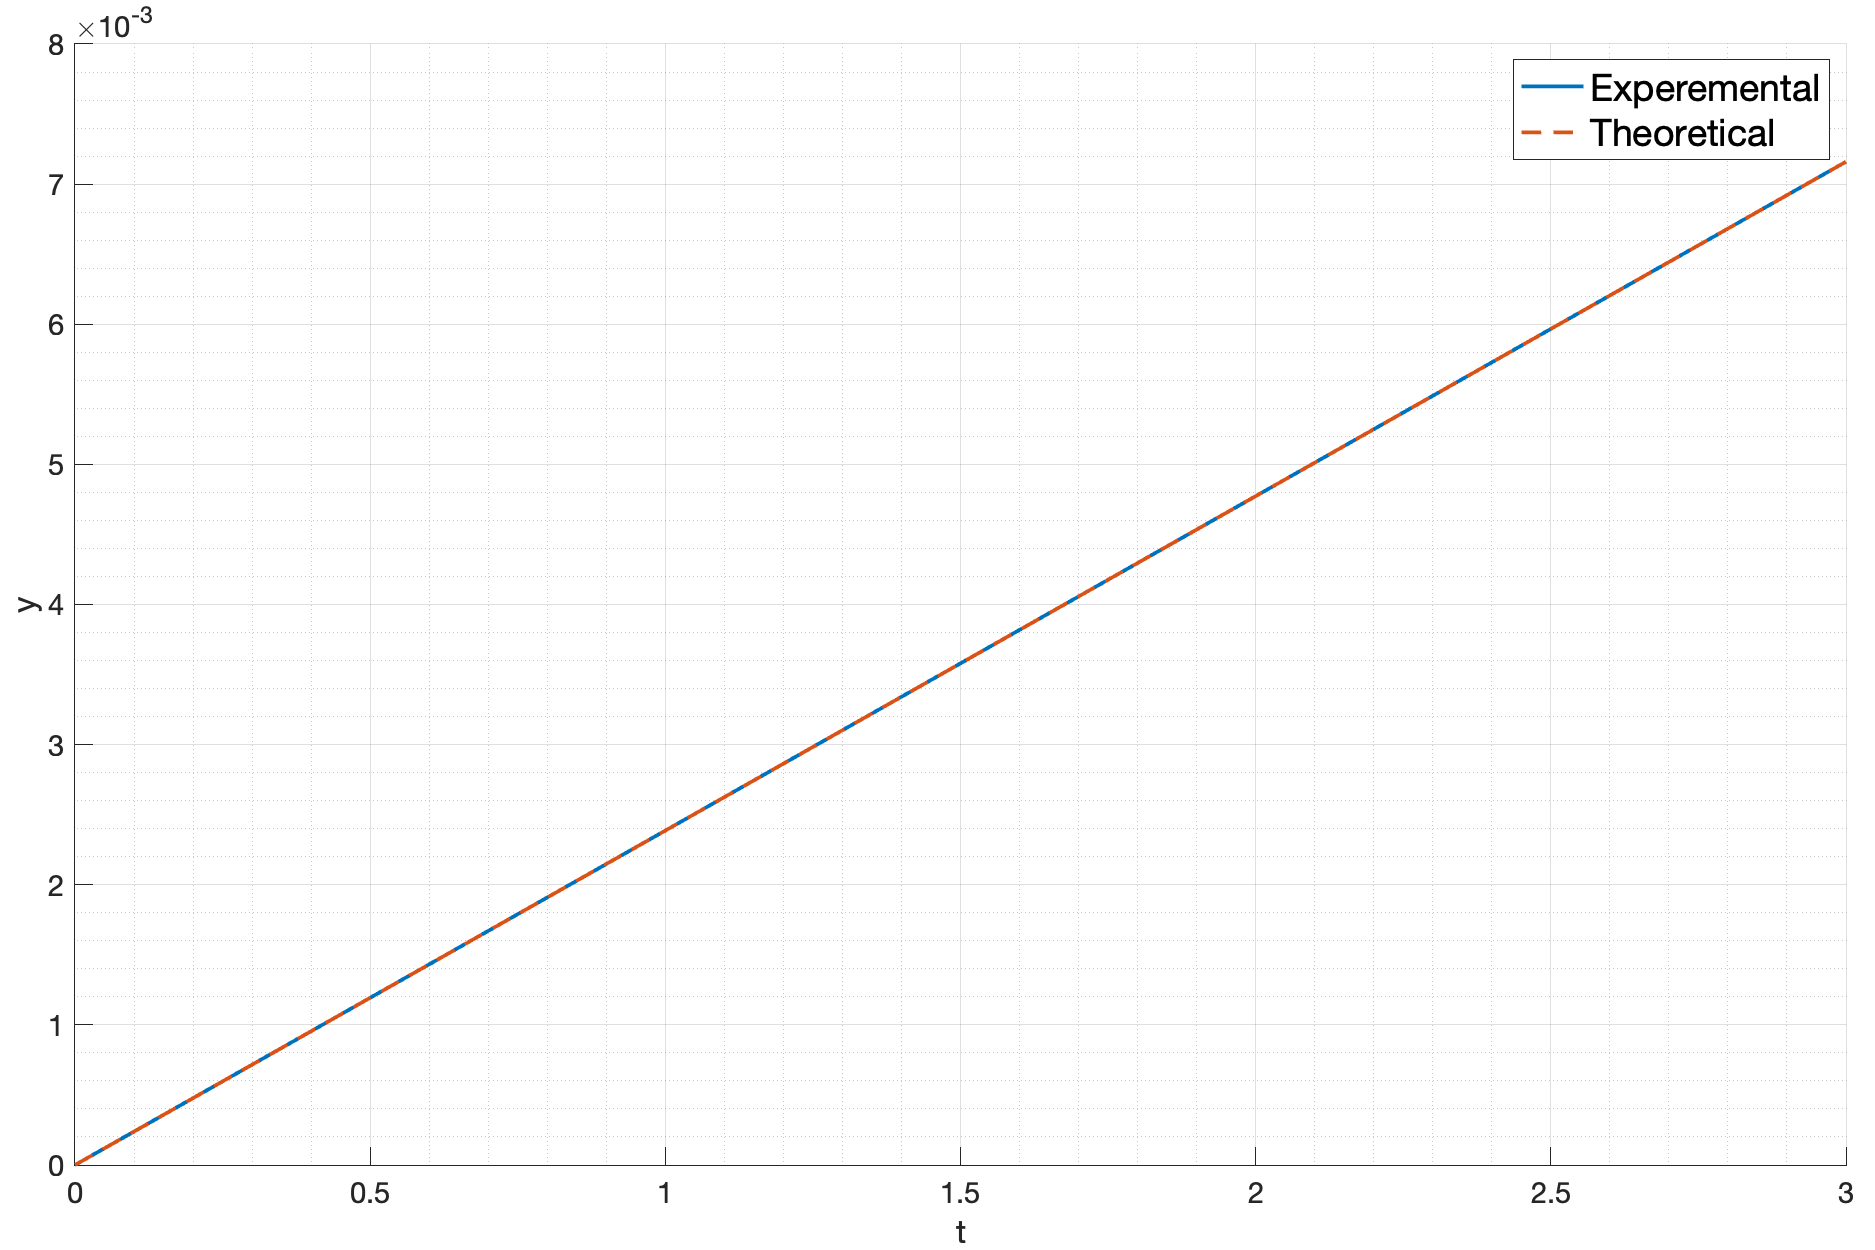
\includegraphics[width=\textwidth]{media/plots/task3_step_response_cmp.png}
    \caption{Сравнение переходных функций конденсатора}
    \label{fig:task3_step_response_cmp}
\end{figure}

\FloatBarrier
\subsection{Частотные характеристики}
\noindent Найдем амплитудно-частотную характеристику и фазо-частотную характеристику,
\begin{equation}
    W(j\omega) = \frac{1}{j\omega C} = -\frac{j}{\omega C}
\end{equation}
Таким образом, АЧХ и ФЧХ системы равны:
\begin{equation}
    A(\omega) = \sqrt{\frac{1}{\omega^2C^2}} = \frac{1}{\omega C}
\end{equation}
\begin{equation}
    \varphi(\omega) = -\frac{\pi}{2}
\end{equation}

Построим графики АЧХ, ФЧХ (см. рис. \ref{fig:task3_freq_resp_eq_lin}) и логарифмическую АЧХ (см. рис. \ref{fig:task3_freq_resp_eq_loglog}).
\begin{figure}[ht!]
    \centering
    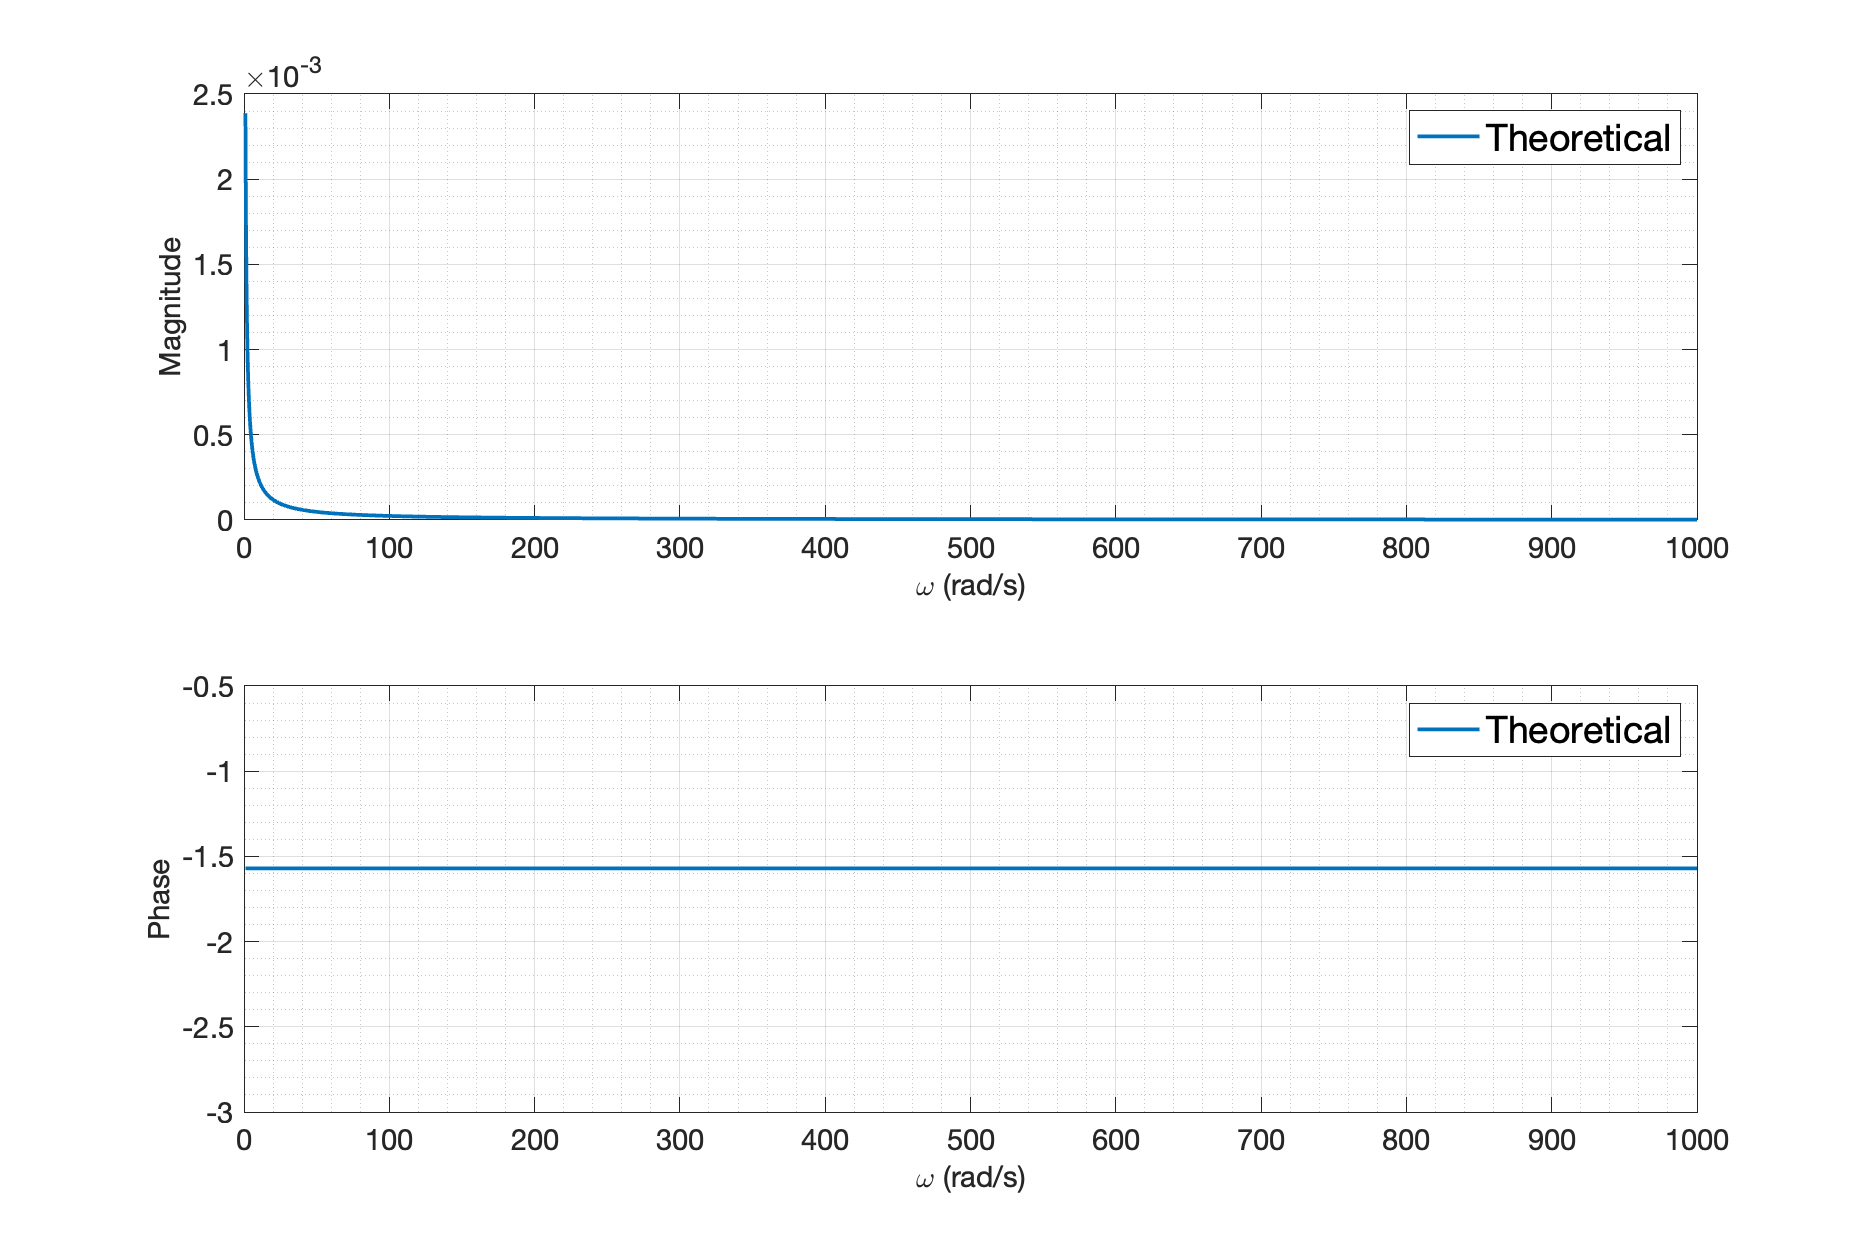
\includegraphics[width=\textwidth]{media/plots/task3_freq_resp_eq_lin.png}
    \caption{АЧХ и ФЧХ конденсатора (теоретически)}
    \label{fig:task3_freq_resp_eq_lin}
\end{figure}
\begin{figure}[ht!]
    \centering
    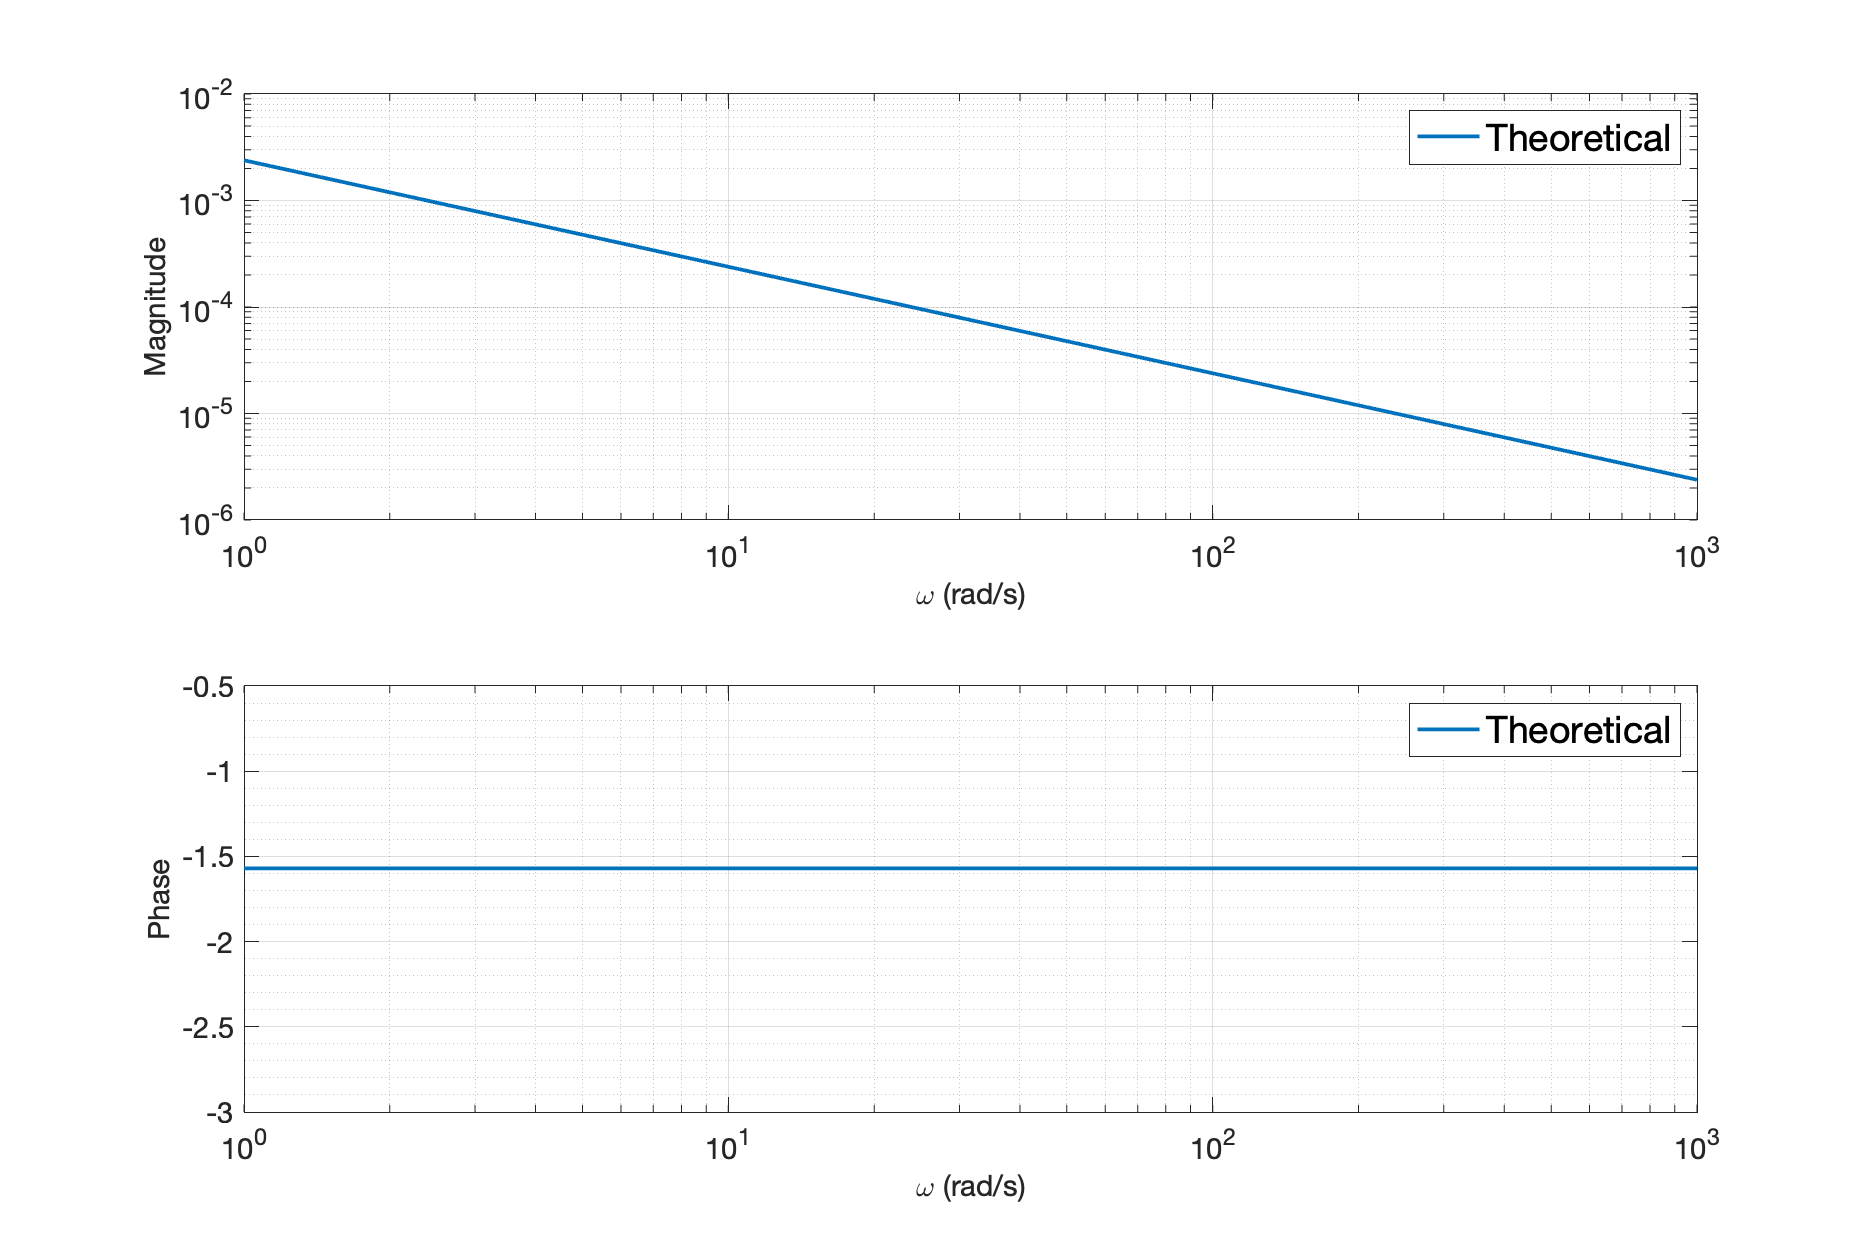
\includegraphics[width=\textwidth]{media/plots/task3_freq_resp_eq_loglog.png}
    \caption{Логарифмическая АЧХ конденсатора (теоретически)}
    \label{fig:task3_freq_resp_eq_loglog}
\end{figure}

AЧХ, ФЧХ и логарифмическая АЧХ, полученные в результате моделирования приведены на рис. \ref{fig:task2_freq_resp_exp_lin} и рис. \ref{fig:task2_freq_resp_exp_loglog}.
\begin{figure}[ht!]
    \centering
    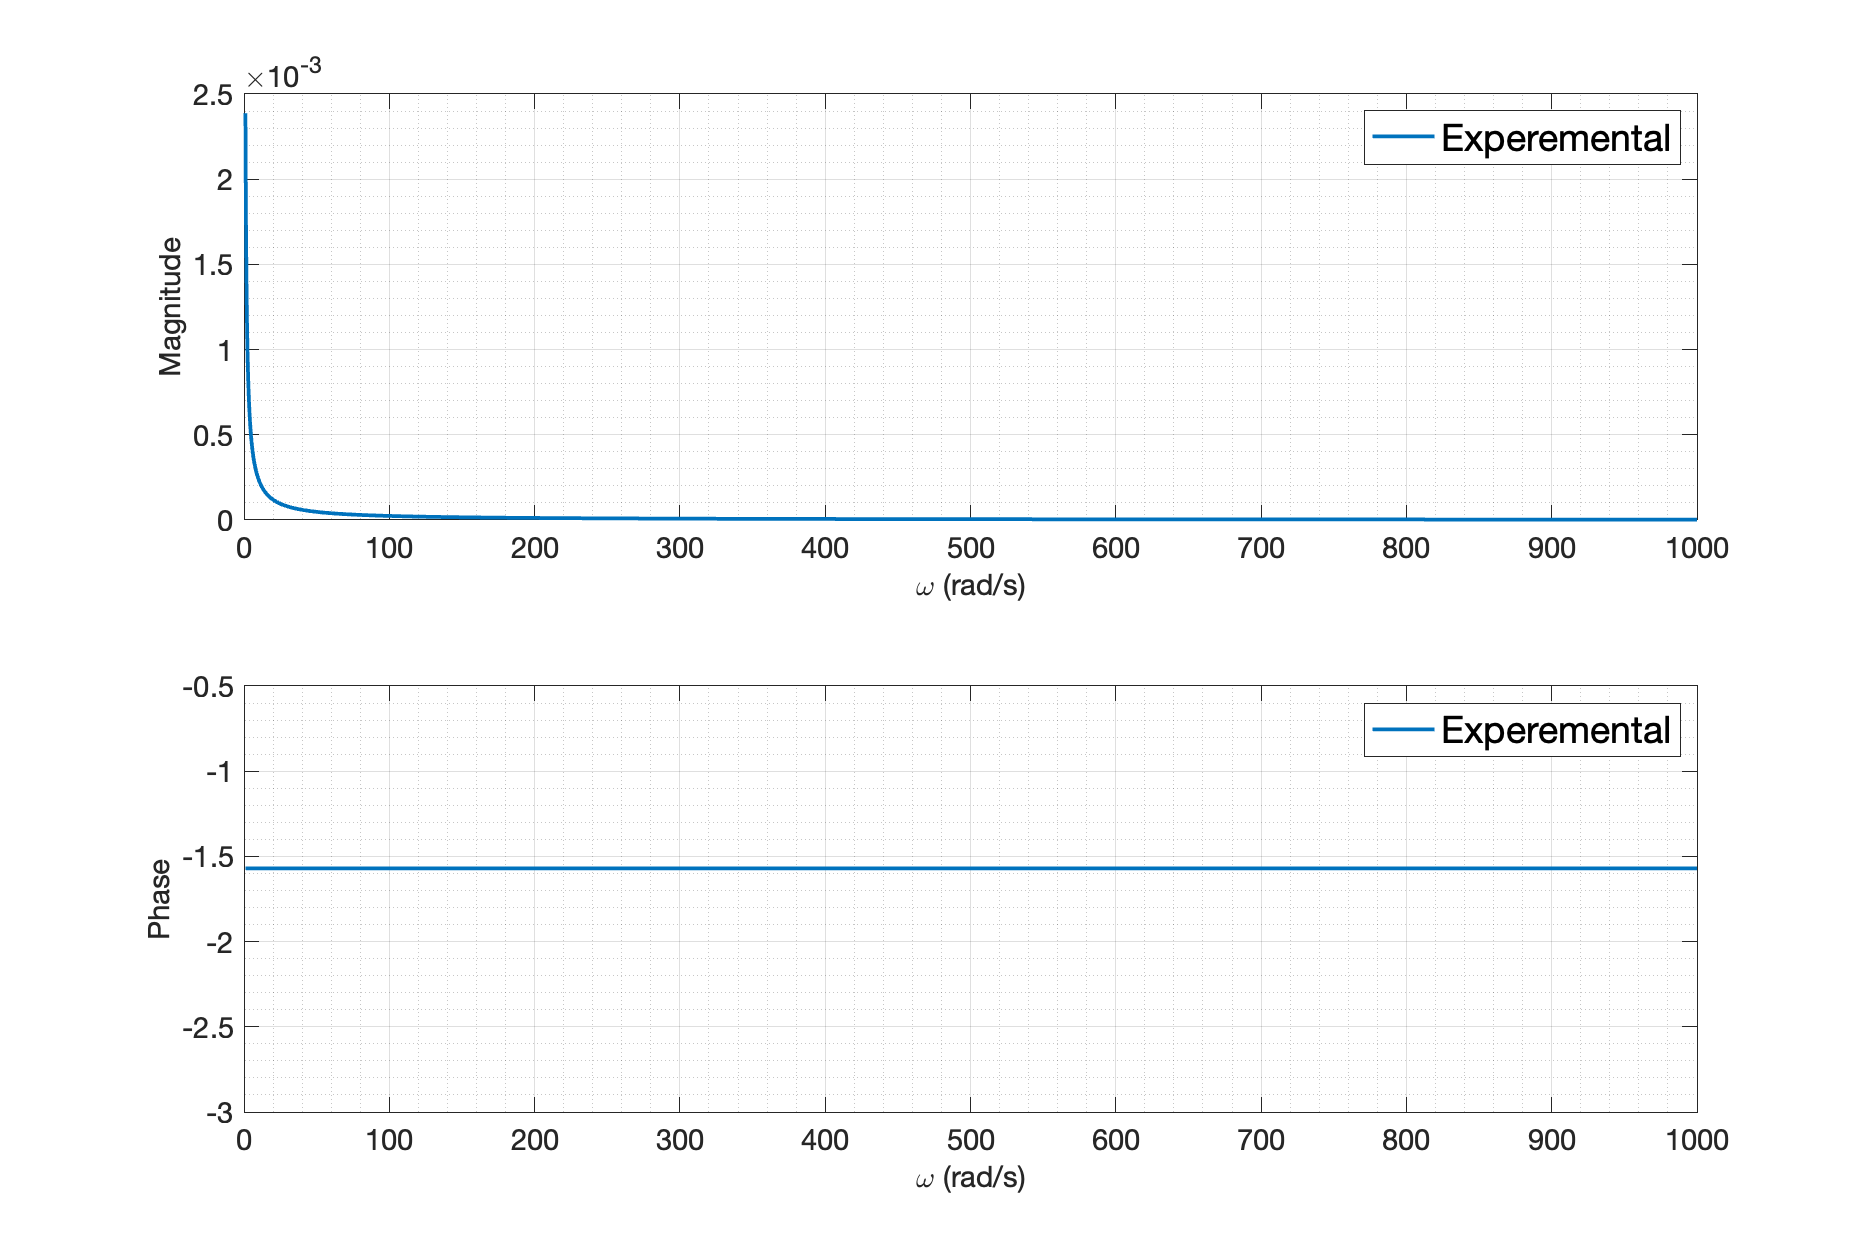
\includegraphics[width=\textwidth]{media/plots/task3_freq_resp_exp_lin.png}
    \caption{АЧХ и ФЧХ конденсатора (экспериментально)}
    \label{fig:task3_freq_resp_exp_lin}
\end{figure}
\begin{figure}[ht!]
    \centering
    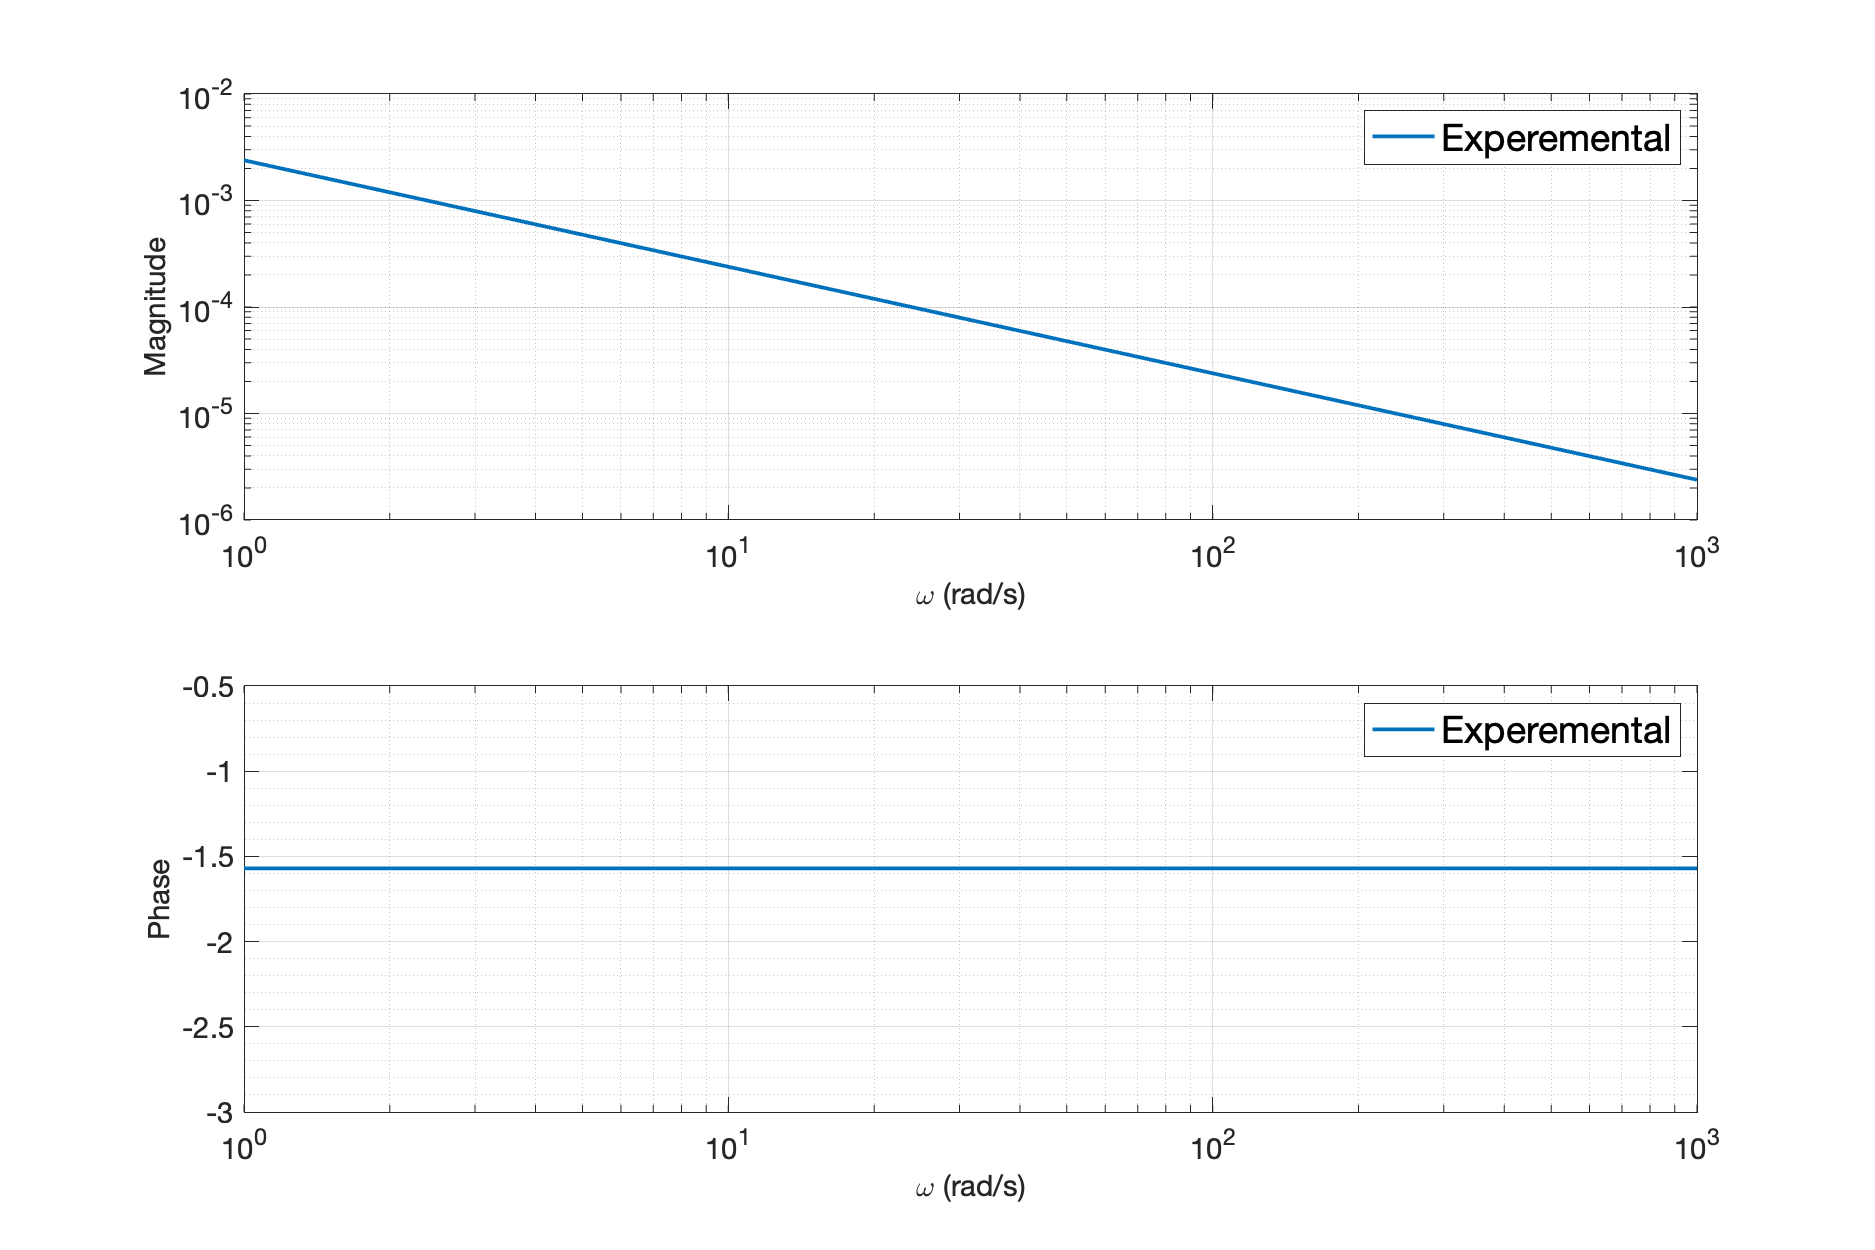
\includegraphics[width=\textwidth]{media/plots/task3_freq_resp_exp_loglog.png}
    \caption{Логарифмическая АЧХ конденсатора (экспериментально)}
    \label{fig:task3_freq_resp_exp_loglog}
\end{figure}

Сравнительные графики приведены на рис. \ref{fig:task3_freq_resp_cmp_lin} и рис. \ref{fig:task3_freq_resp_cmp_loglog}.
\begin{figure}[ht!]
    \centering
    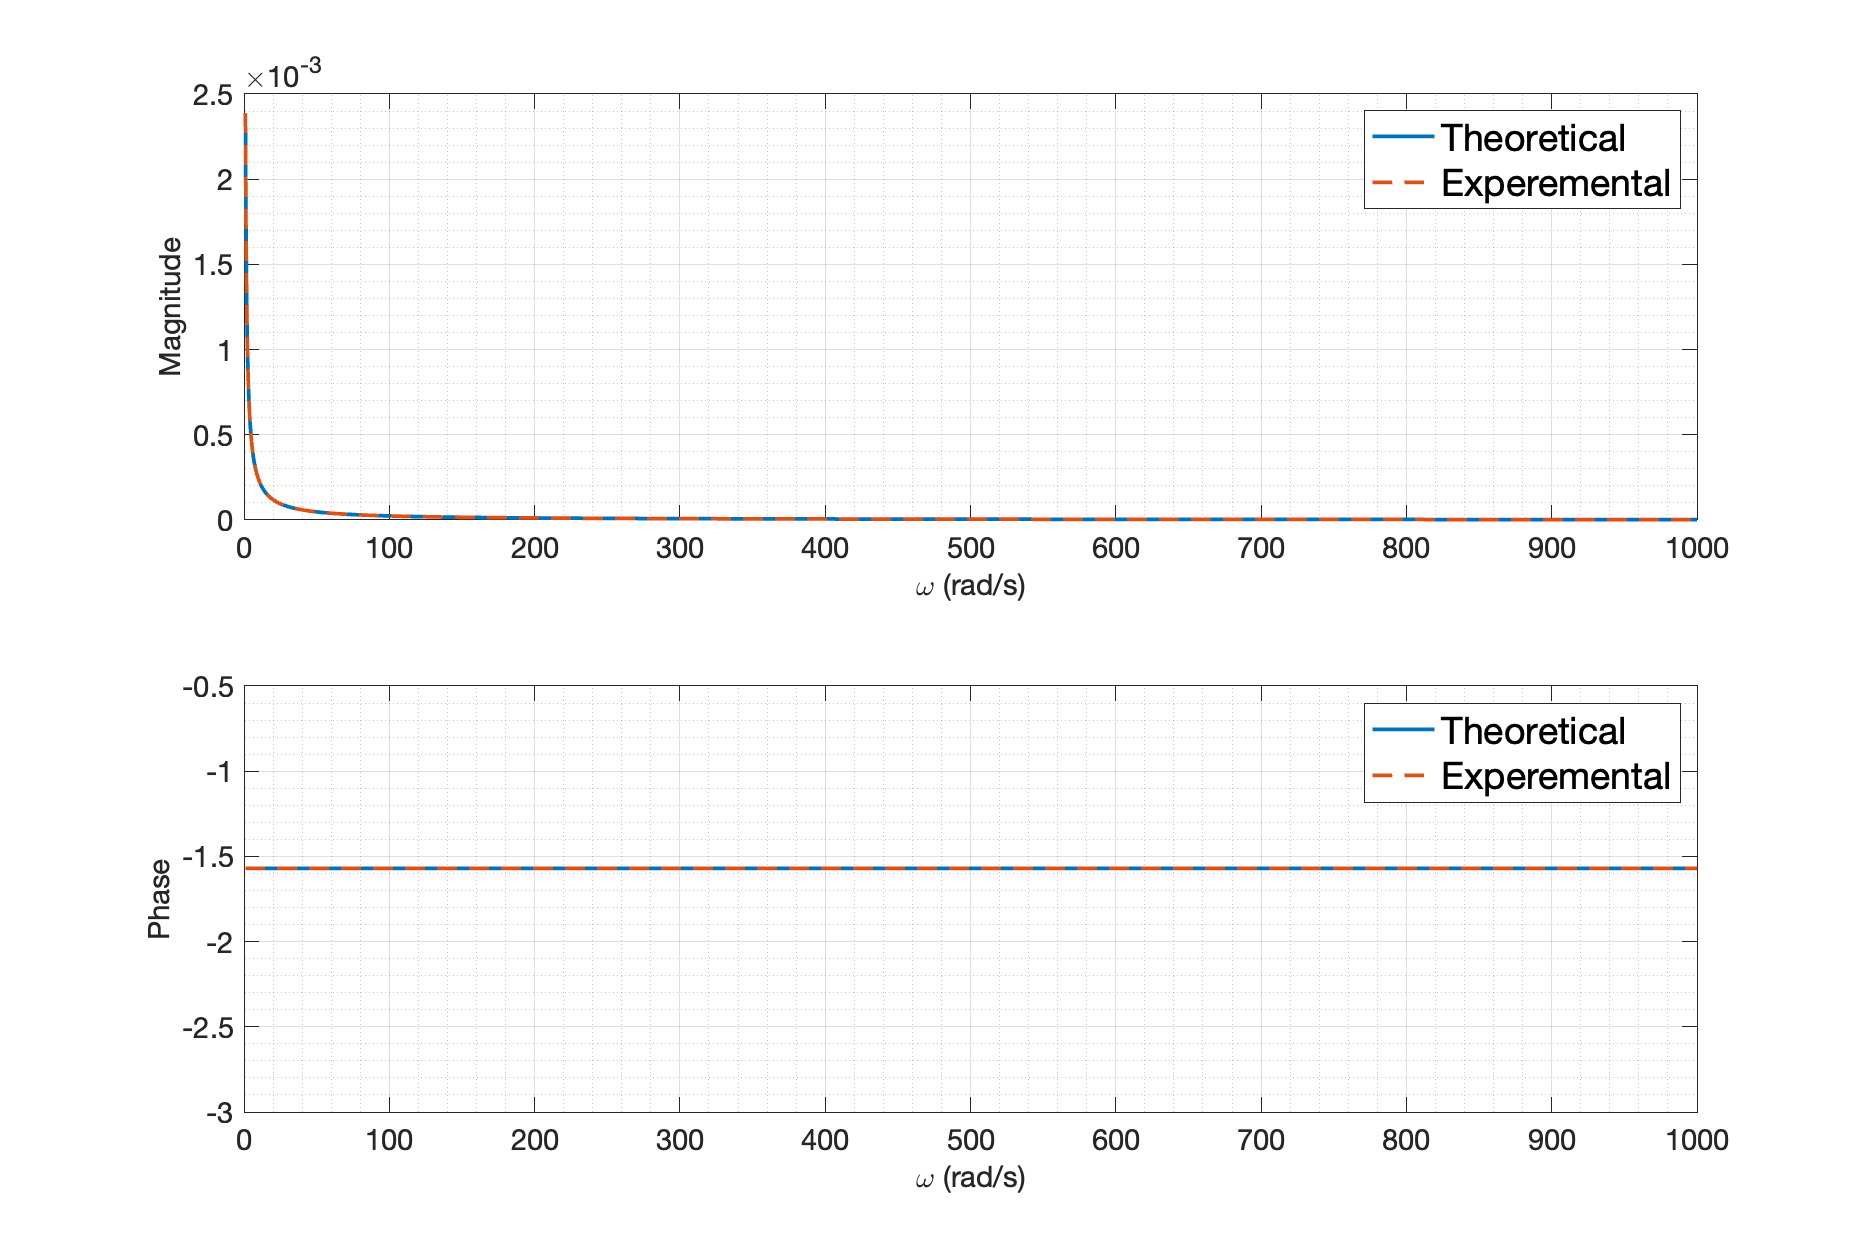
\includegraphics[width=\textwidth]{media/plots/task3_freq_resp_cmp_lin.png}
    \caption{Сравнение АЧХ и ФЧХ конденсатора}
    \label{fig:task3_freq_resp_cmp_lin}
\end{figure}
\begin{figure}[ht!]
    \centering
    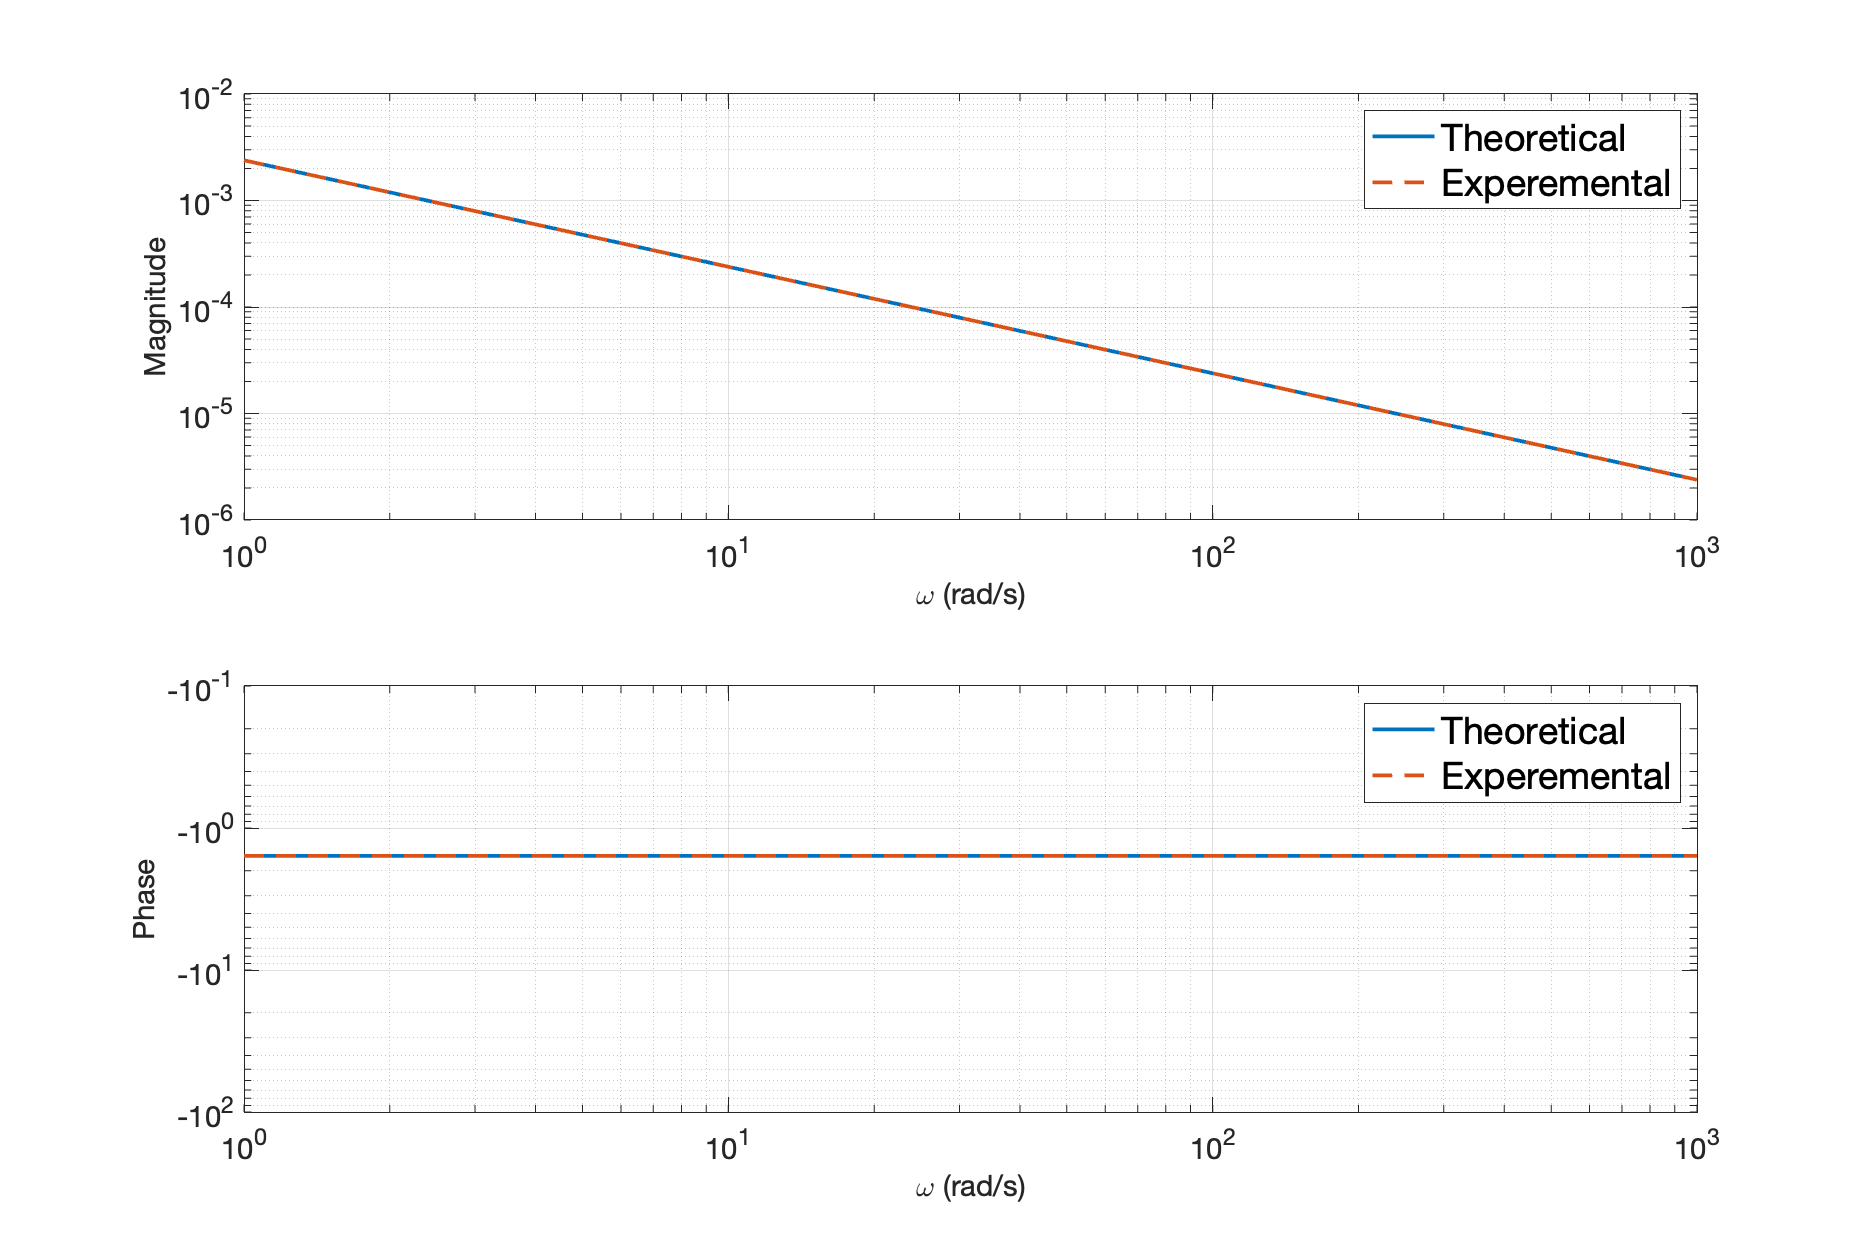
\includegraphics[width=\textwidth]{media/plots/task3_freq_resp_cmp_loglog.png}
    \caption{Сравнение логарифмической АЧХ конденсатора}
    \label{fig:task3_freq_resp_cmp_loglog}
\end{figure}

